\section{Auswertung}
\label{sec:Auswertung}
In \autoref{fig:kennlinie1} und \autoref{fig:kennlinie2} sind die fünf gemessenen Kennlinien der Hochvakuumdiode
aufgetragen. Aus Gründen der Lesbarkeit wurden die Kennlinien auf zwei Plots aufgeteilt. Die dazu entsprechenden
Messwerte sind im Anhang zu finden. Der Sättigungswert wird als Maximum der Kennlinie bestimmt. Insgesamt fällt
auf, dass alle bis auf die Kennlinie für die maximale Heizstromstärke $I_{\symup{H}}=\SI{2,5}{\ampere}$ den zu
erwartenen Verlauf aufweisen. Daraus lässt sich folgern, dass der Sättigungswert hier nur als grobe Näherung
betrachtet werden kann. Die Sättigungswerte sind in \autoref{tab:saettigungswerte} dargestellt.
\begin{figure}
  \centering
  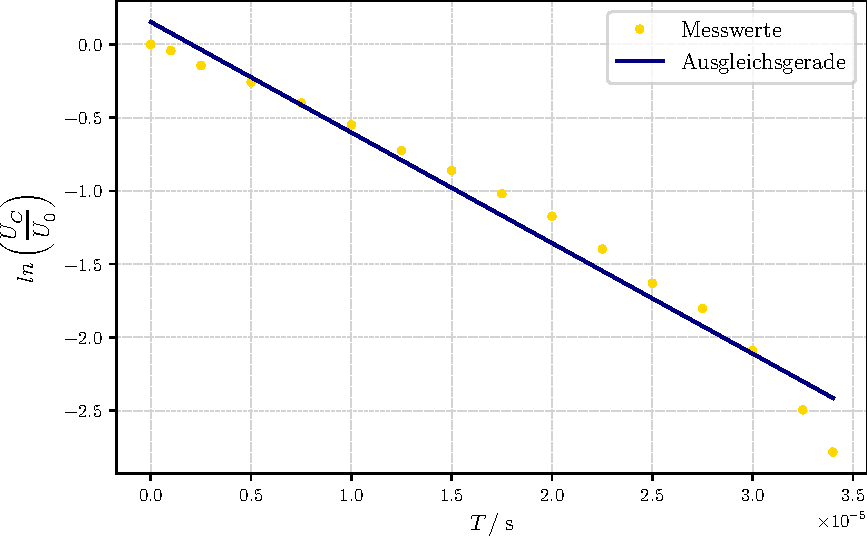
\includegraphics{plot1.pdf}
  \caption{Zwei Kennlinien der Hochvakuumdiode.}
  \label{fig:kennlinie1}
\end{figure}

\begin{figure}
  \centering
  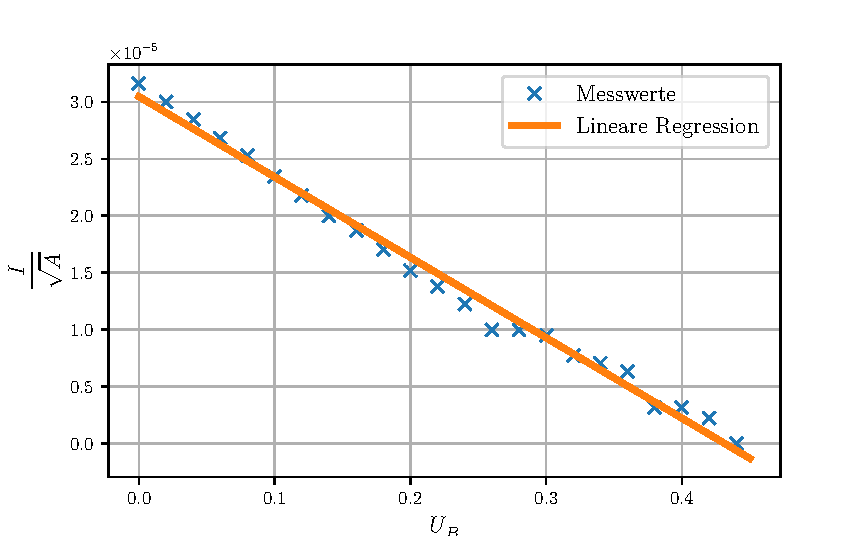
\includegraphics{plot2.pdf}
  \caption{Drei Kennlinien der Hochvakuumdiode.}
  \label{fig:kennlinie2}
\end{figure}
\begin{table}
  \centering
  \caption{Sättigungswerte der Kennlinien}
  \label{tab:saettigungswerte}
  \begin{tabular}{c c}
    \toprule
    $I_{\symup{H}}/\si{\ampere}$ & $I_{\symup{S}}/\si{\milli\ampere}$ \\
    \midrule
    1,9 & 0,052 \\
    2,0 & 0,199 \\
    2,1 & 0,294 \\
    2,3 & 1,289 \\
    2,5 & 3,020 \\
    \bottomrule
  \end{tabular}
\end{table}

\subsection{Gültigkeit des Langmuir-Schottkyschen Raumladungsgesetzes}
\label{sec:Langmuir}
\autoref{eqn:Langmuir} hat die Form $I=\bar{b}U^{m}$ und lässt sich durch logarithmisieren in eine
Geradengleichung der Form
\begin{equation*}
  log(I) = mlog(U)+b
\end{equation*}
mit $b = log(\bar{b})$ bringen. Die Gültigkeit der Gleichung wird nun mit den Messwerten der Kennlinie mit der
höchsten Heizstromstärke $I_{\symup{H}}=\SI{2,5}{\ampere}$ mit Hilfe einer linearen Regression überprüft.
Die logarithmisierten Werte und die lineare Regression sind in \autoref{fig:plot3} dargestellt.
\begin{figure}
  \centering
  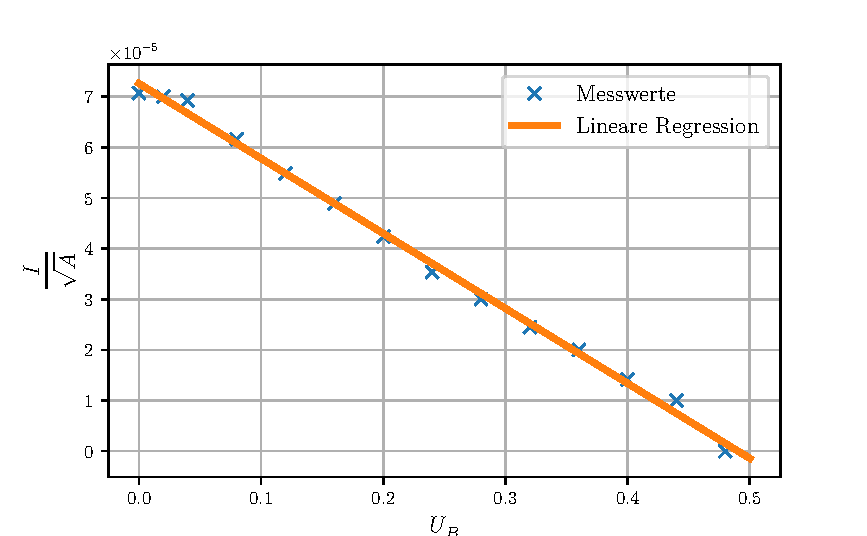
\includegraphics{plot3.pdf}
  \caption{logarithmisierte Kennlinie für $I_{\symup{H}}=\SI{2,5}{\ampere}$ und die entsprechende lineare
  Regression}
  \label{fig:plot3}
\end{figure}
Die Parameter der linearen Regression bestimmen sich zu
\begin{align*}
  m &= 1,439 \pm 0008 \\
  b &= -6,802 \pm 0,037\,.
\end{align*}
$b$ ist dabei für die Auswertung vernachlässigbar. Nur $m$ kann durch den Theoriewert von $m_{\symup{Theo}}=
\frac{3}{2}$ zur Bestimmung der Gültigkeit des Langmuir-Schottkyschen Raumladungsgesetzes verwendet werden.

\subsection{Bestimmung der Kathodentemperatur}
\label{sec:kathodetemp}
